\documentclass[11pt,letterpaper,oneside]{report}

%% =============================================================================
%% PACKAGES
%% =============================================================================

% Page geometry and layout
\usepackage[margin=1in]{geometry}
\usepackage{fancyhdr}
\usepackage{setspace}

% Typography and fonts
\usepackage[T1]{fontenc}
\usepackage{lmodern}
\usepackage{microtype}

% Colors and graphics
\usepackage[dvipsnames,svgnames,x11names]{xcolor}
\usepackage{graphicx}
\usepackage{tikz}
\usetikzlibrary{shapes.geometric, arrows.meta, positioning, fit, backgrounds, calc}

% Code listings
\usepackage{listings}
\usepackage{inconsolata}

% Tables
\usepackage{booktabs}
\usepackage{longtable}
\usepackage{array}
\usepackage{tabularx}
\usepackage{multirow}

% Lists and formatting
\usepackage{enumitem}
\usepackage{parskip}

% Boxes and callouts
\usepackage[most]{tcolorbox}

% Math (for any technical notation)
\usepackage{amsmath}
\usepackage{amssymb}

% Cross-references and hyperlinks (load late)
\usepackage[hypertexnames=false]{hyperref}
\usepackage[capitalise,noabbrev]{cleveref}
%% =============================================================================
%% COLOR DEFINITIONS
%% =============================================================================

\definecolor{primaryblue}{RGB}{0,82,147}
\definecolor{accentorange}{RGB}{230,126,34}
\definecolor{lightgray}{RGB}{248,248,248}
\definecolor{darkgray}{RGB}{60,60,60}
\definecolor{successgreen}{RGB}{39,174,96}
\definecolor{warningred}{RGB}{192,57,43}
\definecolor{codebg}{RGB}{245,245,245}
\definecolor{codeframe}{RGB}{200,200,200}

% Syntax highlighting colors
\definecolor{keyword}{RGB}{0,0,180}
\definecolor{string}{RGB}{163,21,21}
\definecolor{comment}{RGB}{0,128,0}
\definecolor{identifier}{RGB}{0,0,0}
\definecolor{number}{RGB}{128,0,128}

%% =============================================================================
%% LISTINGS CONFIGURATION
%% =============================================================================

\lstset{
    basicstyle=\ttfamily\small,
    backgroundcolor=\color{codebg},
    frame=single,
    rulecolor=\color{codeframe},
    framesep=5pt,
    xleftmargin=10pt,
    xrightmargin=10pt,
    breaklines=true,
    breakatwhitespace=true,
    showstringspaces=false,
    tabsize=2,
    captionpos=b,
    numbers=left,
    numberstyle=\tiny\color{gray},
    numbersep=8pt,
    keywordstyle=\color{keyword}\bfseries,
    stringstyle=\color{string},
    commentstyle=\color{comment}\itshape,
    identifierstyle=\color{identifier},
}

% C language definition
\lstdefinelanguage{C}{
    morekeywords={auto,break,case,char,const,continue,default,do,double,else,enum,
        extern,float,for,goto,if,inline,int,long,register,restrict,return,short,
        signed,sizeof,static,struct,switch,typedef,union,unsigned,void,volatile,
        while,_Bool,_Complex,_Imaginary,_Static_assert,offsetof,NULL,true,false},
    sensitive=true,
    morecomment=[s]{/*}{*/},
    morecomment=[l]//,
    morestring=[b]",
    morestring=[b]',
}

% Bash language definition
\lstdefinelanguage{bash}{
    morekeywords={if,then,else,elif,fi,for,while,do,done,case,esac,function,
        return,in,select,until,local,declare,typeset,readonly,export,unset,
        shift,set,shopt,source,exit,exec,eval,cd,pwd,echo,printf,read,test,
        mkdir,rm,cp,mv,chmod,chown,git,make,jq,opa,grep},
    sensitive=true,
    morecomment=[l]\#,
    morestring=[b]",
    morestring=[b]',
    alsoletter={-},
}

% YAML language definition
\lstdefinelanguage{yaml}{
    keywords={true,false,null,y,n},
    sensitive=false,
    comment=[l]{\#},
    morestring=[b]',
    morestring=[b]",
    moredelim=[l][\color{accentorange}]{:\ },
    moredelim=[l][\color{primaryblue}]{-\ },
}

% Rego language definition
\lstdefinelanguage{rego}{
    morekeywords={package,import,default,as,with,not,some,every,if,contains,else},
    sensitive=true,
    morecomment=[l]\#,
    morestring=[b]",
}

% JSON language definition
\lstdefinelanguage{json}{
    morestring=[b]",
    literate=
        *{:}{{{\color{accentorange}:}}}{1}
        {,}{{{\color{darkgray},}}}{1}
        {\{}{{{\color{primaryblue}\{}}}{1}
        {\}}{{{\color{primaryblue}\}}}}{1}
        {[}{{{\color{primaryblue}[}}}{1}
        {]}{{{\color{primaryblue}]}}}{1},
}

% Makefile language
\lstdefinelanguage{makefile}{
    morekeywords={include,ifdef,ifndef,ifeq,ifneq,else,endif,define,endef,
        override,export,unexport,vpath},
    sensitive=true,
    morecomment=[l]\#,
    morestring=[b]",
    morestring=[b]',
}

%% =============================================================================
%% TCOLORBOX ENVIRONMENTS
%% =============================================================================

% Important note box
\newtcolorbox{importantbox}[1][]{
    colback=warningred!5,
    colframe=warningred!75!black,
    fonttitle=\bfseries,
    title={\faExclamationTriangle\ Important},
    #1
}

% Tip box
\newtcolorbox{tipbox}[1][]{
    colback=successgreen!5,
    colframe=successgreen!75!black,
    fonttitle=\bfseries,
    title={Tip},
    #1
}

% Info box
\newtcolorbox{infobox}[1][]{
    colback=primaryblue!5,
    colframe=primaryblue!75!black,
    fonttitle=\bfseries,
    title={Note},
    #1
}

% Definition box
\newtcolorbox{definitionbox}[2][]{
    colback=lightgray,
    colframe=darkgray,
    fonttitle=\bfseries,
    title={#2},
    #1
}

%% =============================================================================
%% HEADER/FOOTER CONFIGURATION
%% =============================================================================

\pagestyle{fancy}
\fancyhf{}
\fancyhead[L]{\leftmark}
\fancyhead[R]{\thepage}
\fancyfoot[C]{\small Schreiner OOC CI/CD Blueprint}
\renewcommand{\headrulewidth}{0.4pt}
\renewcommand{\footrulewidth}{0.4pt}

\setlength{\headheight}{14pt}
%% =============================================================================
%% HYPERREF CONFIGURATION
%% =============================================================================

\hypersetup{
    colorlinks=true,
    linkcolor=primaryblue,
    urlcolor=accentorange,
    citecolor=successgreen,
    pdftitle={Schreiner OOC-in-C: Enterprise CI/CD Blueprint},
    pdfauthor={},
    pdfsubject={CI/CD Pipeline Architecture for Object-Oriented C},
    pdfkeywords={CI/CD, GitHub Actions, OOC, C Programming, Static Analysis},
    bookmarksnumbered=true,
    bookmarksopen=true,
}

%% =============================================================================
%% CUSTOM COMMANDS
%% =============================================================================

\newcommand{\code}[1]{\texttt{\small #1}}
\newcommand{\filepath}[1]{\texttt{\small\color{accentorange}#1}}
\newcommand{\cmdline}[1]{\texttt{\small\$ #1}}
\newcommand{\envvar}[1]{\texttt{\small\$\{#1\}}}

%% =============================================================================
%% DOCUMENT
%% =============================================================================

\begin{document}

%% -----------------------------------------------------------------------------
%% TITLE PAGE
%% -----------------------------------------------------------------------------

\begin{titlepage}
    \centering
    \vspace*{2cm}
    
    {\huge\bfseries\color{primaryblue} Schreiner OOC-in-C}\\[0.5cm]
    {\LARGE\bfseries Enterprise CI/CD Blueprint}\\[1cm]
    
    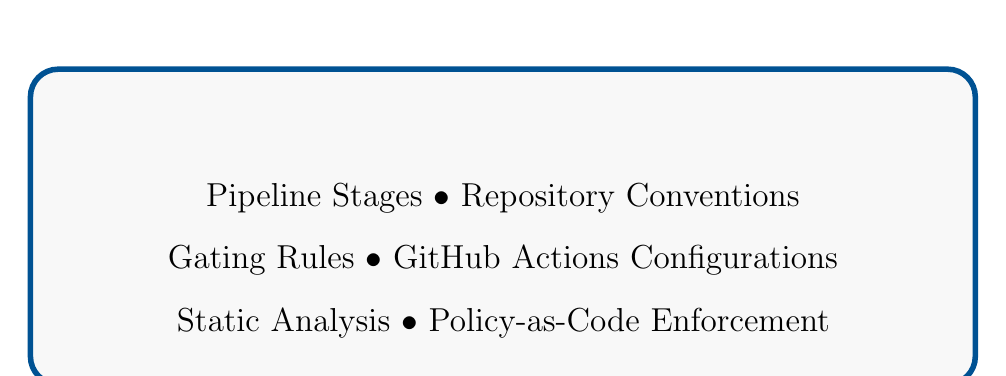
\begin{tikzpicture}
        \node[draw=primaryblue, line width=2pt, rounded corners=10pt, 
              minimum width=12cm, minimum height=4cm, fill=lightgray] (box) {};
        \node[above=0.5cm] at (box.south) {
            \begin{minipage}{10cm}
                \centering
                \large
                Pipeline Stages $\bullet$ Repository Conventions\\[0.3cm]
                Gating Rules $\bullet$ GitHub Actions Configurations\\[0.3cm]
                Static Analysis $\bullet$ Policy-as-Code Enforcement
            \end{minipage}
        };
    \end{tikzpicture}
    
    \vspace{1.5cm}
    
    {\Large Enforceable, Organization-Wide Quality Gates for\\
    Object-Oriented Programming in ANSI C}
    
    \vfill
    
    \begin{tikzpicture}
        \draw[primaryblue, line width=1pt] (0,0) -- (10,0);
    \end{tikzpicture}
    
    \vspace{0.5cm}
    
    {\large\today}
    
    \vspace{1cm}
    
    {\small Version 1.0}
    
\end{titlepage}

%% -----------------------------------------------------------------------------
%% TABLE OF CONTENTS
%% -----------------------------------------------------------------------------

\tableofcontents
\newpage

%% -----------------------------------------------------------------------------
%% EXECUTIVE SUMMARY
%% -----------------------------------------------------------------------------

\chapter*{Executive Summary}
\addcontentsline{toc}{chapter}{Executive Summary}

This document presents a comprehensive, implementation-ready CI/CD blueprint for enforcing Schreiner-style Object-Oriented Programming in ANSI C (OOC) across an organization's C projects. The architecture transforms coding conventions from mere guidelines into \textbf{enforceable gates} that prevent non-compliant code from reaching production.

\section*{Key Deliverables}

\begin{itemize}[leftmargin=*]
    \item \textbf{Repository Contracts}: Standardized directory layouts with compiler-enforced encapsulation through opaque types
    \item \textbf{Automated Code Generation}: Deterministic ooc preprocessor integration with drift detection
    \item \textbf{Static Analysis Gates}: Custom verification scripts targeting Schreiner's invariants plus compile-time assertions
    \item \textbf{Policy-as-Code}: Open Policy Agent (OPA) rules for structural validation
    \item \textbf{Reusable Workflows}: Centralized GitHub Actions configurations consumable by all repositories
    \item \textbf{Organization Rulesets}: Hard gates that prevent bypass through branch protection
\end{itemize}

\section*{Enforcement Philosophy}

The blueprint follows a ``defense in depth'' strategy:

\begin{enumerate}[leftmargin=*]
    \item \textbf{Compile-time enforcement}: \code{\_Static\_assert} macros catch vtable and inheritance violations before code runs
    \item \textbf{Structural verification}: Scripts validate header exposure, layering, and completeness
    \item \textbf{Policy validation}: OPA ensures architectural rules are met
    \item \textbf{Runtime verification}: Sanitizers (ASan/UBSan) catch memory and undefined behavior issues
    \item \textbf{Mandatory review}: CODEOWNERS ensures specialist oversight of critical changes
\end{enumerate}

%% =============================================================================
%% PART I: SINGLE REPOSITORY IMPLEMENTATION
%% =============================================================================

\part{Single Repository Implementation}

\chapter{Repository Architecture}
\label{ch:repo-architecture}

\section{Directory Layout Design}
\label{sec:directory-layout}

The recommended repository structure separates concerns while making CI gates straightforward to implement. This layout accommodates Schreiner's class definitions, method specifications, and the clear separation between public APIs and private implementations.

\begin{lstlisting}[language=bash,caption={Recommended OOC Repository Structure},label={lst:repo-structure}]
project-root/
  src/
    ooc/
      classes/
        Point.d           # Class description file
        Point.ms          # Method specification file
        Shape.d
        Shape.ms
        Circle.d
        Circle.ms
      runtime/
        Object.h          # Base object header
        Object.c          # Base object implementation
        Class.h           # Class descriptor header
        Class.c           # Class descriptor implementation
        ooc_assert.h      # Compile-time assertion macros
      include/
        ooc/              # PUBLIC headers (opaque types + APIs)
          Point.h
          Shape.h
          Circle.h
      internal/
        ooc/              # PRIVATE headers (struct layouts, vtables)
          Point_priv.h
          Shape_priv.h
          Circle_priv.h
  tests/
    unit/
      test_point.c
      test_shape.c
      test_circle.c
    integration/
  scripts/
    ooc-gen.sh            # Code generation script
    ooc-verify.sh         # Structural verification script
    changed-files-json.sh # Policy input generator
  policy/
    ooc.rego              # OPA policy rules
  tools/
    ooc/                  # ooc preprocessor tool
      ooc                 # Main entry point
  build/
    gen/                  # Generated code output
    obj/                  # Object files
    bin/                  # Executables
  .github/
    workflows/
      ci.yml
    CODEOWNERS
\end{lstlisting}

\section{Compiler-Enforced Encapsulation}
\label{sec:encapsulation}

The most robust way to enforce ``no direct struct-member access'' is to make violations \textbf{non-compilable} through opaque types. External code attempting to access structure members receives a compiler error because the structure definition is incomplete.

\subsection{Public Header Pattern}

Public headers declare types as opaque pointers and expose only the API:

\begin{lstlisting}[language=C,caption={Public Header: \filepath{src/ooc/include/ooc/Point.h}},label={lst:public-header}]
/**
 * @file Point.h
 * @brief Public API for Point class (opaque type)
 * 
 * This header provides the public interface to the Point class.
 * The internal structure is hidden to enforce encapsulation.
 */

#pragma once

#ifdef __cplusplus
extern "C" {
#endif

/* Opaque type declaration - struct definition is hidden */
typedef struct Point Point;

/**
 * @brief Create a new Point instance
 * @param x The x-coordinate
 * @param y The y-coordinate
 * @return Pointer to newly allocated Point, or NULL on failure
 */
Point* Point_new(int x, int y);

/**
 * @brief Get the x-coordinate of a Point
 * @param self Pointer to the Point instance
 * @return The x-coordinate value
 */
int Point_x(const Point* self);

/**
 * @brief Get the y-coordinate of a Point
 * @param self Pointer to the Point instance
 * @return The y-coordinate value
 */
int Point_y(const Point* self);

/**
 * @brief Set the x-coordinate of a Point
 * @param self Pointer to the Point instance
 * @param x New x-coordinate value
 */
void Point_setX(Point* self, int x);

/**
 * @brief Set the y-coordinate of a Point
 * @param self Pointer to the Point instance
 * @param y New y-coordinate value
 */
void Point_setY(Point* self, int y);

/**
 * @brief Move a Point by the specified offsets
 * @param self Pointer to the Point instance
 * @param dx Offset in the x direction
 * @param dy Offset in the y direction
 */
void Point_move(Point* self, int dx, int dy);

/**
 * @brief Delete a Point instance and free its memory
 * @param self Pointer to the Point instance
 */
void Point_delete(Point* self);

#ifdef __cplusplus
}
#endif
\end{lstlisting}

\subsection{Private Header Pattern}

Private headers contain the actual structure definitions and are only included by the implementation files:

\begin{lstlisting}[language=C,caption={Private Header: \filepath{src/ooc/internal/ooc/Point\_priv.h}},label={lst:private-header}]
/**
 * @file Point_priv.h
 * @brief Private implementation details for Point class
 * 
 * WARNING: This header should ONLY be included by:
 *   - Point.c (the class implementation)
 *   - Derived class private headers
 *   - Unit tests that need to verify internal state
 * 
 * External code must use the public API in Point.h
 */

#pragma once

#include "ooc/Point.h"
#include "ooc/Class.h"
#include "ooc_assert.h"

/**
 * @brief Point structure definition
 * 
 * Invariants:
 *   - 'class' pointer must be first field (for vtable dispatch)
 *   - 'class' must never be NULL after construction
 */
struct Point {
    const struct Class* class;  /* vtable/class pointer - MUST be first */
    int x;                      /* x-coordinate */
    int y;                      /* y-coordinate */
};

/* Compile-time verification of vtable placement */
OOC_ASSERT_VTABLE_FIRST(struct Point, class);

/**
 * @brief Point class descriptor (vtable)
 * 
 * Contains function pointers for virtual methods
 */
extern const struct Class* PointClass;

/**
 * @brief Internal constructor (called by Point_new and derived classes)
 * @param self Pre-allocated Point memory
 * @param x Initial x-coordinate
 * @param y Initial y-coordinate
 * @return Initialized Point pointer
 */
Point* Point_ctor(Point* self, int x, int y);

/**
 * @brief Internal destructor (called by Point_delete and derived classes)
 * @param self Point instance to destroy
 */
void Point_dtor(Point* self);
\end{lstlisting}

\subsection{Derived Class with Structure Lengthening}

Schreiner's ``judicious lengthening of structures'' pattern enables inheritance by placing the base struct as the first field:

\begin{lstlisting}[language=C,caption={Derived Class: \filepath{src/ooc/internal/ooc/Circle\_priv.h}},label={lst:derived-class}]
/**
 * @file Circle_priv.h
 * @brief Private implementation details for Circle class
 * 
 * Circle extends Shape using Schreiner's structure lengthening pattern.
 * The Shape base struct must be the first field to enable safe casting.
 */

#pragma once

#include "ooc/Circle.h"
#include "ooc/internal/ooc/Shape_priv.h"
#include "ooc_assert.h"

/**
 * @brief Circle structure definition (extends Shape)
 * 
 * Inheritance is achieved by placing the base struct first.
 * A Circle* can be safely cast to Shape* and Object*.
 */
struct Circle {
    struct Shape base;    /* Base class - MUST be first field */
    double radius;        /* Circle-specific: radius */
};

/* Compile-time verification of inheritance layout */
OOC_ASSERT_BASE_FIRST(struct Circle, base);

/**
 * @brief Circle class descriptor (vtable)
 */
extern const struct Class* CircleClass;

/**
 * @brief Internal constructor
 */
Circle* Circle_ctor(Circle* self, int x, int y, double radius);

/**
 * @brief Internal destructor
 */
void Circle_dtor(Circle* self);
\end{lstlisting}

\section{Compile-Time Assertion Macros}
\label{sec:static-assertions}

The assertion header provides macros that enforce Schreiner's structural invariants at compile time:

\begin{lstlisting}[language=C,caption={Compile-Time Assertions: \filepath{src/ooc/runtime/ooc\_assert.h}},label={lst:assert-macros}]
/**
 * @file ooc_assert.h
 * @brief Compile-time assertions for OOC structural invariants
 * 
 * These macros enforce Schreiner's OOC patterns at compile time:
 *   - Virtual table pointer must be the first field
 *   - Base struct must be the first field (structure lengthening)
 *   - Size and alignment requirements
 * 
 * Violations result in compilation errors, not runtime failures.
 */

#pragma once

#include <stddef.h>

/**
 * @brief Assert that the vtable/class pointer is the first field
 * 
 * Schreiner's OOC requires the class descriptor pointer to be at
 * offset 0 for virtual dispatch to work correctly.
 * 
 * @param T The struct type (e.g., struct Point)
 * @param field The vtable field name (typically 'class')
 * 
 * Example:
 *   struct Point { const struct Class* class; int x, y; };
 *   OOC_ASSERT_VTABLE_FIRST(struct Point, class);
 */
#define OOC_ASSERT_VTABLE_FIRST(T, field) \
    _Static_assert(offsetof(T, field) == 0, \
        "OOC violation: vtable/class pointer must be first field in " #T)

/**
 * @brief Assert that the base struct is the first field (inheritance)
 * 
 * Structure lengthening requires the base struct to be at offset 0
 * so that derived pointers can be safely cast to base pointers.
 * 
 * @param DerivedT The derived struct type (e.g., struct Circle)
 * @param base_field The base struct field name (typically 'base')
 * 
 * Example:
 *   struct Circle { struct Shape base; double r; };
 *   OOC_ASSERT_BASE_FIRST(struct Circle, base);
 */
#define OOC_ASSERT_BASE_FIRST(DerivedT, base_field) \
    _Static_assert(offsetof(DerivedT, base_field) == 0, \
        "OOC violation: base struct must be first field in " #DerivedT \
        " (structure lengthening requirement)")

/**
 * @brief Assert size relationship between derived and base
 * 
 * A derived struct must be at least as large as its base.
 * 
 * @param DerivedT The derived struct type
 * @param BaseT The base struct type
 */
#define OOC_ASSERT_DERIVED_SIZE(DerivedT, BaseT) \
    _Static_assert(sizeof(DerivedT) >= sizeof(BaseT), \
        "OOC violation: " #DerivedT " must be at least as large as " #BaseT)

/**
 * @brief Assert that a type has no padding at the start
 * 
 * Useful for ensuring binary compatibility in class descriptors.
 * 
 * @param T The struct type
 * @param first_field The name of the first field
 */
#define OOC_ASSERT_NO_INITIAL_PADDING(T, first_field) \
    _Static_assert(offsetof(T, first_field) == 0, \
        "OOC violation: unexpected padding before " #first_field " in " #T)

/**
 * @brief Verify class descriptor initialization
 * 
 * Runtime check (not compile-time) for NULL class pointers.
 * Use in constructors and after allocation.
 * 
 * @param obj Pointer to object
 */
#define OOC_VERIFY_INITIALIZED(obj) \
    do { \
        if ((obj) == NULL || *((const void**)(obj)) == NULL) { \
            fprintf(stderr, "OOC error: uninitialized object at %s:%d\n", \
                    __FILE__, __LINE__); \
            abort(); \
        } \
    } while (0)
\end{lstlisting}

\chapter{Code Generation Integration}
\label{ch:code-generation}

\section{The ooc Preprocessor}
\label{sec:ooc-preprocessor}

Schreiner's ooc tool generates boilerplate code from class descriptions (\code{.d} files) and method specifications (\code{.ms} files). Proper CI integration ensures:

\begin{enumerate}[leftmargin=*]
    \item Generation is \textbf{deterministic} (same inputs always produce same outputs)
    \item Generation \textbf{fails fast} on errors
    \item Generated code is either \textbf{not committed} (preferred) or \textbf{drift-checked}
\end{enumerate}

\section{Generation Script}
\label{sec:generation-script}

\begin{lstlisting}[language=bash,caption={Code Generation Script: \filepath{scripts/ooc-gen.sh}},label={lst:ooc-gen}]
#!/usr/bin/env bash
#
# ooc-gen.sh - Generate OOC boilerplate code
#
# This script invokes the ooc preprocessor to generate headers and
# source files from class descriptions (.d) and method specs (.ms).
#
# Exit codes:
#   0 - Success
#   1 - General error
#   2 - Missing method specification file
#   3 - Missing generated output
#   4 - ooc tool not found

set -euo pipefail

# Determine script and project root directories
SCRIPT_DIR="$(cd "$(dirname "${BASH_SOURCE[0]}")" && pwd)"
ROOT="$(cd "${SCRIPT_DIR}/.." && pwd)"

# Configuration (can be overridden via environment)
SRC="${OOC_SRC_DIR:-${ROOT}/src/ooc/classes}"
OUT="${OOC_OUT_DIR:-${ROOT}/build/gen}"
OOC="${OOC_TOOL:-${ROOT}/tools/ooc/ooc}"

# Logging functions
log_info() { echo "[ooc-gen] INFO: $*"; }
log_error() { echo "[ooc-gen] ERROR: $*" >&2; }

# Verify ooc tool exists
if [[ ! -x "${OOC}" ]]; then
    log_error "ooc tool not found or not executable: ${OOC}"
    log_error "Set OOC_TOOL environment variable to override"
    exit 4
fi

# Create output directory
mkdir -p "${OUT}"

# Track what we generate for verification
declare -a generated_classes=()

# Enable nullglob for safe iteration over potentially empty glob
shopt -s nullglob

# Process each class description file
for d_file in "${SRC}"/*.d; do
    base="$(basename "${d_file}" .d)"
    ms_file="${SRC}/${base}.ms"
    
    # Verify method specification exists
    if [[ ! -f "${ms_file}" ]]; then
        log_error "Missing method specification: ${ms_file}"
        log_error "Each .d file must have a corresponding .ms file"
        exit 2
    fi
    
    log_info "Generating ${base} from ${d_file} and ${ms_file}"
    
    # Invoke ooc preprocessor
    # Adjust flags according to your specific ooc implementation:
    #   -d <file>  : Class description file
    #   -m <file>  : Method specification file
    #   -o <dir>   : Output directory
    #   -h         : Generate header
    #   -c         : Generate source
    "${OOC}" -d "${d_file}" -m "${ms_file}" -o "${OUT}" -h -c
    
    generated_classes+=("${base}")
done

# Verify all expected outputs were generated
log_info "Verifying generated outputs..."
for base in "${generated_classes[@]}"; do
    header="${OUT}/${base}.h"
    source="${OUT}/${base}.c"
    
    if [[ ! -f "${header}" ]]; then
        log_error "Missing generated header: ${header}"
        exit 3
    fi
    
    if [[ ! -f "${source}" ]]; then
        log_error "Missing generated source: ${source}"
        exit 3
    fi
    
    log_info "  Verified: ${base}.h, ${base}.c"
done

log_info "Generation complete: ${#generated_classes[@]} classes processed"
log_info "Output directory: ${OUT}"
\end{lstlisting}

\section{Drift Detection}
\label{sec:drift-detection}

If your organization commits generated code (for debugging or review purposes), add drift detection to ensure the committed version matches what the generator produces:

\begin{lstlisting}[language=bash,caption={Drift Detection Check},label={lst:drift-check}]
#!/usr/bin/env bash
#
# check-drift.sh - Verify generated code hasn't drifted from source
#
set -euo pipefail

SCRIPT_DIR="$(cd "$(dirname "${BASH_SOURCE[0]}")" && pwd)"

# Run generation
"${SCRIPT_DIR}/ooc-gen.sh"

# Check for differences
if ! git diff --exit-code -- build/gen; then
    echo "ERROR: Generated code has drifted from committed version" >&2
    echo "Please run ./scripts/ooc-gen.sh and commit the results" >&2
    exit 1
fi

echo "Generated code is up to date"
\end{lstlisting}

\chapter{Static Analysis and Verification}
\label{ch:static-analysis}

\section{Compiler-Driven Gates}
\label{sec:compiler-gates}

The first line of defense is strict compiler flags applied to \textbf{all builds}:

\begin{lstlisting}[language=bash,caption={Recommended Compiler Flags},label={lst:compiler-flags}]
# Base flags (always applied)
CFLAGS_BASE = -std=c11 -Wall -Wextra -Wpedantic -Werror

# Extended warnings (recommended)
CFLAGS_EXTENDED = \
    -Wshadow \
    -Wcast-align \
    -Wstrict-prototypes \
    -Wmissing-prototypes \
    -Wmissing-declarations \
    -Wconversion \
    -Wsign-conversion \
    -Wformat=2 \
    -Wformat-security \
    -Wnull-dereference \
    -Wstack-protector \
    -Wdouble-promotion

# Critical: forbid escape hatches
CFLAGS_STRICT = \
    -Werror=implicit-function-declaration \
    -Werror=return-type \
    -Werror=incompatible-pointer-types

# Combined production flags
CFLAGS = $(CFLAGS_BASE) $(CFLAGS_EXTENDED) $(CFLAGS_STRICT)
\end{lstlisting}

\section{Structural Verification Script}
\label{sec:verify-script}

This script enforces OOC-specific rules that compilers cannot check:

\begin{lstlisting}[language=bash,caption={Structural Verification Script: \filepath{scripts/ooc-verify.sh}},label={lst:ooc-verify}]
#!/usr/bin/env bash
#
# ooc-verify.sh - Verify OOC structural rules
#
# This script enforces conventions that cannot be checked by the compiler:
#   - No concrete struct bodies in public headers
#   - Internal headers only included from implementation
#   - Class file completeness (.d/.ms pairs)
#   - Naming conventions
#
# Exit codes:
#   0  - All checks passed
#   10 - Public header exposes struct body
#   11 - Internal header included from wrong location
#   12 - Missing method specification (.ms) file
#   13 - Naming convention violation

set -euo pipefail

SCRIPT_DIR="$(cd "$(dirname "${BASH_SOURCE[0]}")" && pwd)"
ROOT="$(cd "${SCRIPT_DIR}/.." && pwd)"

# Configuration
PUBLIC_INCLUDE="${ROOT}/src/ooc/include"
INTERNAL_INCLUDE="${ROOT}/src/ooc/internal"
CLASSES_DIR="${ROOT}/src/ooc/classes"
OOC_SRC="${ROOT}/src/ooc"

# Colors for output
RED='\033[0;31m'
GREEN='\033[0;32m'
YELLOW='\033[1;33m'
NC='\033[0m' # No Color

pass() { echo -e "${GREEN}[PASS]${NC} $*"; }
fail() { echo -e "${RED}[FAIL]${NC} $*" >&2; }
warn() { echo -e "${YELLOW}[WARN]${NC} $*"; }

errors=0

echo "=========================================="
echo "OOC Structural Verification"
echo "=========================================="
echo ""

# --------------------------------------------------------------------------
# Check 1: No concrete struct bodies in public headers
# --------------------------------------------------------------------------
echo "Checking: Public headers must use opaque types..."

# Pattern matches: struct SomeName { (with whitespace variations)
# This catches struct definitions, not just declarations
if grep -r --include='*.h' -l -E '^\s*struct\s+[A-Za-z_][A-Za-z0-9_]*\s*\{' \
    "${PUBLIC_INCLUDE}" 2>/dev/null; then
    
    fail "Public headers contain struct bodies (use opaque types)"
    echo ""
    echo "Violations found in:"
    grep -r --include='*.h' -n -E '^\s*struct\s+[A-Za-z_][A-Za-z0-9_]*\s*\{' \
        "${PUBLIC_INCLUDE}" || true
    echo ""
    echo "Fix: Move struct definitions to internal headers"
    echo "     Public headers should only have: typedef struct Name Name;"
    errors=$((errors + 1))
else
    pass "Public headers use opaque types only"
fi
echo ""

# --------------------------------------------------------------------------
# Check 2: Internal headers only included from OOC implementation
# --------------------------------------------------------------------------
echo "Checking: Internal headers not exposed outside OOC..."

# Find includes of internal headers from outside src/ooc/
bad_includes=$(grep -r --include='*.c' --include='*.h' \
    -l -E '#include\s+["<].*internal.*[">]' "${ROOT}/src" 2>/dev/null | \
    grep -v "^${OOC_SRC}/" || true)

if [[ -n "${bad_includes}" ]]; then
    fail "Internal headers included from outside OOC implementation"
    echo ""
    echo "Violations:"
    echo "${bad_includes}" | while read -r f; do
        echo "  ${f}:"
        grep -n -E '#include\s+["<].*internal.*[">]' "${f}" | \
            sed 's/^/    /'
    done
    errors=$((errors + 1))
else
    pass "Internal headers properly encapsulated"
fi
echo ""

# --------------------------------------------------------------------------
# Check 3: Every .d file has a corresponding .ms file
# --------------------------------------------------------------------------
echo "Checking: Class completeness (.d/.ms pairs)..."

shopt -s nullglob
missing_ms=0
for d_file in "${CLASSES_DIR}"/*.d; do
    base="$(basename "${d_file}" .d)"
    ms_file="${CLASSES_DIR}/${base}.ms"
    
    if [[ ! -f "${ms_file}" ]]; then
        fail "Missing method spec: ${base}.ms for ${base}.d"
        missing_ms=$((missing_ms + 1))
    fi
done

if [[ ${missing_ms} -eq 0 ]]; then
    pass "All class descriptions have method specifications"
else
    errors=$((errors + missing_ms))
fi
echo ""

# --------------------------------------------------------------------------
# Check 4: Every .d file has a public header
# --------------------------------------------------------------------------
echo "Checking: Public headers exist for all classes..."

missing_headers=0
for d_file in "${CLASSES_DIR}"/*.d; do
    base="$(basename "${d_file}" .d)"
    header="${PUBLIC_INCLUDE}/ooc/${base}.h"
    
    if [[ ! -f "${header}" ]]; then
        fail "Missing public header: ooc/${base}.h for ${base}.d"
        missing_headers=$((missing_headers + 1))
    fi
done

if [[ ${missing_headers} -eq 0 ]]; then
    pass "All classes have public headers"
else
    errors=$((errors + missing_headers))
fi
echo ""

# --------------------------------------------------------------------------
# Check 5: Naming conventions
# --------------------------------------------------------------------------
echo "Checking: Naming conventions..."

# Class names should be PascalCase
naming_errors=0
for d_file in "${CLASSES_DIR}"/*.d; do
    base="$(basename "${d_file}" .d)"
    
    # Check if name starts with uppercase and follows PascalCase
    if ! echo "${base}" | grep -qE '^[A-Z][a-zA-Z0-9]*$'; then
        fail "Class name not PascalCase: ${base}"
        naming_errors=$((naming_errors + 1))
    fi
done

if [[ ${naming_errors} -eq 0 ]]; then
    pass "All class names follow PascalCase convention"
else
    errors=$((errors + naming_errors))
fi
echo ""

# --------------------------------------------------------------------------
# Summary
# --------------------------------------------------------------------------
echo "=========================================="
if [[ ${errors} -eq 0 ]]; then
    echo -e "${GREEN}All checks passed${NC}"
    exit 0
else
    echo -e "${RED}${errors} error(s) found${NC}"
    exit 10
fi
\end{lstlisting}

\section{Memory Safety with Sanitizers}
\label{sec:sanitizers}

Address Sanitizer (ASan) and Undefined Behavior Sanitizer (UBSan) catch memory errors and undefined behavior at runtime:

\begin{lstlisting}[language=makefile,caption={Makefile Sanitizer Targets},label={lst:sanitizer-makefile}]
# Sanitizer flags
SANITIZE_FLAGS = -fsanitize=address,undefined \
                 -fno-omit-frame-pointer \
                 -fno-sanitize-recover=all

# Debug build with sanitizers
.PHONY: sanitize
sanitize: CFLAGS += $(SANITIZE_FLAGS)
sanitize: LDFLAGS += $(SANITIZE_FLAGS)
sanitize: all

# Run tests with sanitizers
.PHONY: test-sanitize
test-sanitize: sanitize
	./bin/test_runner

# Valgrind target (slower, more thorough)
.PHONY: valgrind
valgrind: debug
	valgrind --leak-check=full \
	         --show-leak-kinds=all \
	         --track-origins=yes \
	         --verbose \
	         ./bin/test_runner
\end{lstlisting}

\chapter{Policy-as-Code with Open Policy Agent}
\label{ch:policy-opa}

\section{Policy Architecture}
\label{sec:policy-architecture}

Open Policy Agent (OPA) validates structural and architectural rules using declarative Rego policies. The CI pipeline generates JSON input describing changed files, then OPA evaluates policies against this input.

\begin{figure}[htbp]
\centering
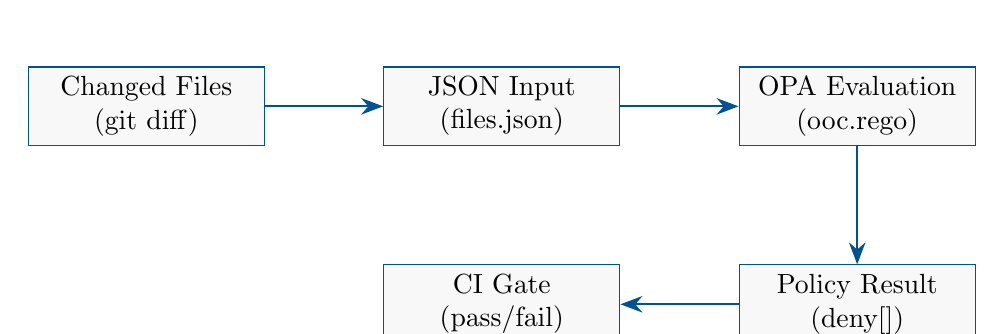
\begin{tikzpicture}[
    node distance=1.5cm,
    box/.style={rectangle, draw=primaryblue, fill=lightgray, 
                minimum width=3cm, minimum height=1cm, align=center},
    arrow/.style={-{Stealth[scale=1.2]}, thick, primaryblue}
]
    % Nodes
    \node[box] (changed) {Changed Files\\(git diff)};
    \node[box, right=of changed] (json) {JSON Input\\(files.json)};
    \node[box, right=of json] (opa) {OPA Evaluation\\(ooc.rego)};
    \node[box, below=of opa] (result) {Policy Result\\(deny[])};
    \node[box, left=of result] (gate) {CI Gate\\(pass/fail)};
    
    % Arrows
    \draw[arrow] (changed) -- (json);
    \draw[arrow] (json) -- (opa);
    \draw[arrow] (opa) -- (result);
    \draw[arrow] (result) -- (gate);
\end{tikzpicture}
\caption{OPA Policy Evaluation Flow}
\label{fig:opa-flow}
\end{figure}

\section{Input Generation Script}
\label{sec:input-generation}

\begin{lstlisting}[language=bash,caption={Policy Input Generator: \filepath{scripts/changed-files-json.sh}},label={lst:changed-files}]
#!/usr/bin/env bash
#
# changed-files-json.sh - Generate JSON input for OPA policy evaluation
#
# Outputs a JSON object with the list of changed files relative to main branch.
# Used by CI to feed OPA for policy validation.
#
set -euo pipefail

OUTPUT_DIR="${1:-build/policy}"
mkdir -p "${OUTPUT_DIR}"

# Ensure we have the main branch for comparison
git fetch origin main --depth=1 2>/dev/null || true

# Get list of changed files
changed_files=$(git diff --name-only origin/main...HEAD 2>/dev/null || \
                git diff --name-only HEAD~1 2>/dev/null || \
                find . -name '*.c' -o -name '*.h' -o -name '*.d' -o -name '*.ms' | \
                sed 's|^\./||')

# Convert to JSON array
echo "${changed_files}" | \
    jq -R -s -c 'split("\n") | map(select(length > 0)) | {files: .}' \
    > "${OUTPUT_DIR}/files.json"

echo "Generated ${OUTPUT_DIR}/files.json"
cat "${OUTPUT_DIR}/files.json"
\end{lstlisting}

\section{OPA Policy Rules}
\label{sec:opa-rules}

\begin{lstlisting}[language=rego,caption={OPA Policy: \filepath{policy/ooc.rego}},label={lst:opa-rego}]
# ooc.rego - OOC Structural Policy Rules
#
# This policy enforces:
#   1. Every class description (.d) has a method spec (.ms)
#   2. Every class has a public header
#   3. Internal headers are in the correct location
#   4. Naming conventions are followed
#
# Usage:
#   opa eval -i files.json -d ooc.rego "data.ooc.deny"

package ooc

import future.keywords.in
import future.keywords.every
import future.keywords.contains
import future.keywords.if

# Default: no denials
default allow := true

# Helper: set of all files
fileset contains f if {
    f := input.files[_]
}

# Extract class names from .d files
classes contains name if {
    some file in input.files
    endswith(file, ".d")
    parts := split(file, "/")
    filename := parts[count(parts) - 1]
    name := trim_suffix(filename, ".d")
}

# Rule 1: Every .d file must have a corresponding .ms file
deny contains msg if {
    some class_name in classes
    expected_ms := sprintf("src/ooc/classes/%s.ms", [class_name])
    not expected_ms in fileset
    
    # Only enforce if the .d file was changed
    changed_d := sprintf("src/ooc/classes/%s.d", [class_name])
    changed_d in fileset
    
    msg := sprintf("Class '%s' is missing method specification: %s", 
                   [class_name, expected_ms])
}

# Rule 2: Every .d file must have a public header
deny contains msg if {
    some class_name in classes
    expected_header := sprintf("src/ooc/include/ooc/%s.h", [class_name])
    not expected_header in fileset
    
    # Only enforce if the .d file was changed
    changed_d := sprintf("src/ooc/classes/%s.d", [class_name])
    changed_d in fileset
    
    msg := sprintf("Class '%s' is missing public header: %s", 
                   [class_name, expected_header])
}

# Rule 3: Private headers must be in internal directory
deny contains msg if {
    some file in input.files
    endswith(file, "_priv.h")
    not startswith(file, "src/ooc/internal/")
    
    msg := sprintf("Private header in wrong location: %s (should be in src/ooc/internal/)", 
                   [file])
}

# Rule 4: Class names must be PascalCase
deny contains msg if {
    some class_name in classes
    not regex.match(`^[A-Z][a-zA-Z0-9]*$`, class_name)
    
    msg := sprintf("Class name '%s' violates PascalCase convention", [class_name])
}

# Rule 5: No .c files directly in src/ooc/include
deny contains msg if {
    some file in input.files
    endswith(file, ".c")
    startswith(file, "src/ooc/include/")
    
    msg := sprintf("Source file in include directory: %s", [file])
}

# Rule 6: Internal headers should have corresponding private header naming
internal_headers contains file if {
    some file in input.files
    startswith(file, "src/ooc/internal/")
    endswith(file, ".h")
}

# Aggregate all denials
violations := deny

# Final result
result := {
    "allow": count(deny) == 0,
    "violations": deny,
    "classes_checked": classes,
    "files_analyzed": count(input.files)
}
\end{lstlisting}

\chapter{Automated Testing}
\label{ch:testing}

\section{Unit Testing Patterns}
\label{sec:unit-testing}

Tests should verify both the API contract and the OOC-specific invariants (polymorphism, type identity, lifecycle):

\begin{lstlisting}[language=C,caption={Unit Test Example: \filepath{tests/unit/test\_circle.c}},label={lst:unit-test}]
/**
 * @file test_circle.c
 * @brief Unit tests for Circle class
 *
 * Tests verify:
 *   - Construction and destruction
 *   - Accessor methods
 *   - Polymorphic dispatch through Shape interface
 *   - Type identity (isA, classOf)
 *   - Memory safety (run with sanitizers)
 */

#include "ooc/Object.h"
#include "ooc/Shape.h"
#include "ooc/Circle.h"
#include <assert.h>
#include <math.h>
#include <stdio.h>
#include <stdlib.h>

/* Tolerance for floating-point comparison */
#define EPSILON 0.0001
#define APPROX_EQ(a, b) (fabs((a) - (b)) < EPSILON)

/* Test framework macros */
#define TEST(name) static void test_##name(void)
#define RUN_TEST(name) do { \
    printf("  Running %s...", #name); \
    test_##name(); \
    printf(" PASSED\n"); \
} while (0)

/* --------------------------------------------------------------------------
 * Test: Basic construction and destruction
 * -------------------------------------------------------------------------- */
TEST(circle_new_delete) {
    Circle* c = Circle_new(10, 20, 5.0);
    assert(c != NULL);
    
    /* Verify initial state */
    assert(Circle_x(c) == 10);
    assert(Circle_y(c) == 20);
    assert(APPROX_EQ(Circle_radius(c), 5.0));
    
    Circle_delete(c);
    /* If we get here without ASan errors, memory management is correct */
}

/* --------------------------------------------------------------------------
 * Test: Polymorphic area() dispatch through Shape interface
 * -------------------------------------------------------------------------- */
TEST(circle_area_polymorphism) {
    /* Create Circle but reference through Shape pointer */
    Shape* s = (Shape*)Circle_new(0, 0, 2.0);
    assert(s != NULL);
    
    /* Call Shape_area - should dispatch to Circle's implementation */
    double area = Shape_area(s);
    double expected = 4.0 * M_PI;  /* pi * r^2 = pi * 4 */
    
    assert(APPROX_EQ(area, expected));
    
    /* Delete through base pointer - tests destructor dispatch */
    Object_delete((Object*)s);
}

/* --------------------------------------------------------------------------
 * Test: Type identity using isA and classOf
 * -------------------------------------------------------------------------- */
TEST(circle_type_identity) {
    Circle* c = Circle_new(0, 0, 1.0);
    
    /* classOf should return the Circle class descriptor */
    const void* class = classOf(c);
    assert(class != NULL);
    
    /* isA should return true for Circle and all ancestors */
    assert(isA(c, Circle));
    assert(isA(c, Shape));
    assert(isA(c, Object));
    
    /* isA should return false for unrelated types */
    /* (assuming Rectangle is another Shape subclass) */
    /* assert(!isA(c, Rectangle)); */
    
    Circle_delete(c);
}

/* --------------------------------------------------------------------------
 * Test: Move operation (inherited from Shape)
 * -------------------------------------------------------------------------- */
TEST(circle_move) {
    Circle* c = Circle_new(10, 10, 3.0);
    
    Shape_move((Shape*)c, 5, -3);
    
    assert(Circle_x(c) == 15);
    assert(Circle_y(c) == 7);
    /* Radius should be unchanged */
    assert(APPROX_EQ(Circle_radius(c), 3.0));
    
    Circle_delete(c);
}

/* --------------------------------------------------------------------------
 * Test: Multiple instances are independent
 * -------------------------------------------------------------------------- */
TEST(circle_multiple_instances) {
    Circle* c1 = Circle_new(0, 0, 1.0);
    Circle* c2 = Circle_new(10, 10, 2.0);
    Circle* c3 = Circle_new(20, 20, 3.0);
    
    /* Modify one, others unchanged */
    Circle_setRadius(c2, 5.0);
    
    assert(APPROX_EQ(Circle_radius(c1), 1.0));
    assert(APPROX_EQ(Circle_radius(c2), 5.0));
    assert(APPROX_EQ(Circle_radius(c3), 3.0));
    
    /* Delete in non-creation order to test memory management */
    Circle_delete(c2);
    Circle_delete(c1);
    Circle_delete(c3);
}

/* --------------------------------------------------------------------------
 * Test: Draw operation (virtual method)
 * -------------------------------------------------------------------------- */
TEST(circle_draw) {
    Shape* shapes[3];
    shapes[0] = (Shape*)Circle_new(0, 0, 1.0);
    shapes[1] = (Shape*)Circle_new(5, 5, 2.0);
    /* shapes[2] = (Shape*)Rectangle_new(10, 10, 3.0, 4.0); */
    shapes[2] = (Shape*)Circle_new(10, 10, 3.0);
    
    /* Polymorphic dispatch - each shape draws itself */
    for (int i = 0; i < 3; i++) {
        Shape_draw(shapes[i]);
        Object_delete((Object*)shapes[i]);
    }
}

/* --------------------------------------------------------------------------
 * Main test runner
 * -------------------------------------------------------------------------- */
int main(void) {
    printf("Circle Unit Tests\n");
    printf("==================\n\n");
    
    RUN_TEST(circle_new_delete);
    RUN_TEST(circle_area_polymorphism);
    RUN_TEST(circle_type_identity);
    RUN_TEST(circle_move);
    RUN_TEST(circle_multiple_instances);
    RUN_TEST(circle_draw);
    
    printf("\nAll tests passed!\n");
    return EXIT_SUCCESS;
}
\end{lstlisting}

\section{Integration Testing}
\label{sec:integration-testing}

Integration tests verify that classes work together correctly:

\begin{lstlisting}[language=C,caption={Integration Test Example},label={lst:integration-test}]
/**
 * @file test_shape_collection.c
 * @brief Integration test for polymorphic shape collections
 */

#include "ooc/Object.h"
#include "ooc/Shape.h"
#include "ooc/Circle.h"
#include "ooc/Rectangle.h"
#include <assert.h>
#include <stdio.h>

void test_heterogeneous_collection(void) {
    /* Create a collection of different shapes */
    Shape* shapes[4];
    shapes[0] = (Shape*)Circle_new(0, 0, 5.0);
    shapes[1] = (Shape*)Rectangle_new(0, 0, 10, 20);
    shapes[2] = (Shape*)Circle_new(10, 10, 3.0);
    shapes[3] = (Shape*)Rectangle_new(5, 5, 8, 8);
    
    /* Calculate total area using polymorphic dispatch */
    double total_area = 0.0;
    for (int i = 0; i < 4; i++) {
        total_area += Shape_area(shapes[i]);
        printf("Shape %d area: %.2f\n", i, Shape_area(shapes[i]));
    }
    printf("Total area: %.2f\n", total_area);
    
    /* Move all shapes */
    for (int i = 0; i < 4; i++) {
        Shape_move(shapes[i], 100, 100);
    }
    
    /* Draw all shapes */
    printf("\nDrawing all shapes:\n");
    for (int i = 0; i < 4; i++) {
        Shape_draw(shapes[i]);
    }
    
    /* Clean up using base class destructor */
    for (int i = 0; i < 4; i++) {
        Object_delete((Object*)shapes[i]);
    }
}

int main(void) {
    test_heterogeneous_collection();
    return 0;
}
\end{lstlisting}

\chapter{GitHub Actions Workflow}
\label{ch:github-actions}

\section{Complete CI Pipeline}
\label{sec:ci-pipeline}

\begin{lstlisting}[language=yaml,caption={GitHub Actions Workflow: \filepath{.github/workflows/ooc-ci.yml}},label={lst:github-actions}]
name: ooc-ci

on:
  pull_request:
    branches: [main, develop]
  push:
    branches: [main]

# Prevent concurrent runs on same branch
concurrency:
  group: ${{ github.workflow }}-${{ github.ref }}
  cancel-in-progress: true

env:
  # Strict compiler flags for all jobs
  CFLAGS_BASE: "-std=c11 -Wall -Wextra -Wpedantic -Werror"

jobs:
  # --------------------------------------------------------------------------
  # Job: Generate OOC boilerplate
  # --------------------------------------------------------------------------
  generate:
    name: ooc/generate
    runs-on: ubuntu-latest
    steps:
      - name: Checkout repository
        uses: actions/checkout@v4
      
      - name: Generate OOC boilerplate
        run: |
          chmod +x scripts/ooc-gen.sh
          ./scripts/ooc-gen.sh
      
      - name: Upload generated sources
        uses: actions/upload-artifact@v4
        with:
          name: generated-sources
          path: build/gen/
          retention-days: 1

  # --------------------------------------------------------------------------
  # Job: Verify OOC structural rules
  # --------------------------------------------------------------------------
  verify:
    name: ooc/verify
    runs-on: ubuntu-latest
    steps:
      - name: Checkout repository
        uses: actions/checkout@v4
      
      - name: Run structural verification
        run: |
          chmod +x scripts/ooc-verify.sh
          ./scripts/ooc-verify.sh

  # --------------------------------------------------------------------------
  # Job: OPA policy validation
  # --------------------------------------------------------------------------
  policy:
    name: ooc/policy
    runs-on: ubuntu-latest
    steps:
      - name: Checkout repository
        uses: actions/checkout@v4
        with:
          fetch-depth: 0  # Need full history for diff
      
      - name: Setup OPA
        uses: open-policy-agent/setup-opa@v2
        with:
          version: latest
      
      - name: Generate policy input
        run: |
          chmod +x scripts/changed-files-json.sh
          ./scripts/changed-files-json.sh build/policy
      
      - name: Evaluate OPA policies
        run: |
          opa eval \
            --input build/policy/files.json \
            --data policy/ooc.rego \
            --format pretty \
            "data.ooc.result" | tee build/policy/result.json
          
          # Extract and check violations
          violations=$(jq '.result[0].expressions[0].value.violations | length' \
                       build/policy/result.json)
          
          if [ "$violations" -gt 0 ]; then
            echo "::error::Policy violations found:"
            jq '.result[0].expressions[0].value.violations[]' \
               build/policy/result.json
            exit 1
          fi
          
          echo "Policy validation passed"
      
      - name: Upload policy results
        if: always()
        uses: actions/upload-artifact@v4
        with:
          name: policy-results
          path: build/policy/
          retention-days: 7

  # --------------------------------------------------------------------------
  # Job: Build with strict warnings
  # --------------------------------------------------------------------------
  build:
    name: ooc/build
    runs-on: ubuntu-latest
    needs: [generate, verify, policy]
    strategy:
      matrix:
        compiler: [gcc, clang]
    steps:
      - name: Checkout repository
        uses: actions/checkout@v4
      
      - name: Download generated sources
        uses: actions/download-artifact@v4
        with:
          name: generated-sources
          path: build/gen/
      
      - name: Install dependencies
        run: |
          sudo apt-get update
          sudo apt-get install -y build-essential ${{ matrix.compiler }}
      
      - name: Build with ${{ matrix.compiler }}
        env:
          CC: ${{ matrix.compiler }}
        run: |
          make clean all \
            CFLAGS="${CFLAGS_BASE} -Wshadow -Wconversion"
      
      - name: Upload build artifacts
        uses: actions/upload-artifact@v4
        with:
          name: build-${{ matrix.compiler }}
          path: |
            build/obj/
            build/bin/
          retention-days: 1

  # --------------------------------------------------------------------------
  # Job: Run unit tests
  # --------------------------------------------------------------------------
  test:
    name: ooc/test
    runs-on: ubuntu-latest
    needs: [build]
    steps:
      - name: Checkout repository
        uses: actions/checkout@v4
      
      - name: Download generated sources
        uses: actions/download-artifact@v4
        with:
          name: generated-sources
          path: build/gen/
      
      - name: Build and run tests
        run: |
          make clean all test \
            CFLAGS="${CFLAGS_BASE}"
      
      - name: Upload test results
        if: always()
        uses: actions/upload-artifact@v4
        with:
          name: test-results
          path: build/test-results/
          retention-days: 7

  # --------------------------------------------------------------------------
  # Job: Sanitizer checks (ASan + UBSan)
  # --------------------------------------------------------------------------
  sanitize:
    name: ooc/sanitize
    runs-on: ubuntu-latest
    needs: [generate, verify, policy]
    steps:
      - name: Checkout repository
        uses: actions/checkout@v4
      
      - name: Download generated sources
        uses: actions/download-artifact@v4
        with:
          name: generated-sources
          path: build/gen/
      
      - name: Build with sanitizers
        env:
          CC: clang
        run: |
          SANITIZE_FLAGS="-fsanitize=address,undefined -fno-omit-frame-pointer"
          make clean all \
            CFLAGS="${CFLAGS_BASE} ${SANITIZE_FLAGS}" \
            LDFLAGS="${SANITIZE_FLAGS}"
      
      - name: Run tests with sanitizers
        env:
          ASAN_OPTIONS: "detect_leaks=1:abort_on_error=1"
          UBSAN_OPTIONS: "print_stacktrace=1:halt_on_error=1"
        run: |
          make test

  # --------------------------------------------------------------------------
  # Job: Valgrind (nightly/main only)
  # --------------------------------------------------------------------------
  valgrind:
    name: ooc/valgrind
    runs-on: ubuntu-latest
    needs: [test]
    if: github.ref == 'refs/heads/main' || github.event_name == 'schedule'
    steps:
      - name: Checkout repository
        uses: actions/checkout@v4
      
      - name: Download generated sources
        uses: actions/download-artifact@v4
        with:
          name: generated-sources
          path: build/gen/
      
      - name: Install Valgrind
        run: |
          sudo apt-get update
          sudo apt-get install -y valgrind
      
      - name: Build debug version
        run: |
          make clean all CFLAGS="${CFLAGS_BASE} -g -O0"
      
      - name: Run Valgrind
        run: |
          valgrind \
            --leak-check=full \
            --show-leak-kinds=all \
            --track-origins=yes \
            --error-exitcode=1 \
            --xml=yes \
            --xml-file=build/valgrind-report.xml \
            ./build/bin/test_runner
      
      - name: Upload Valgrind report
        if: always()
        uses: actions/upload-artifact@v4
        with:
          name: valgrind-report
          path: build/valgrind-report.xml
          retention-days: 30
\end{lstlisting}

\section{CODEOWNERS Configuration}
\label{sec:codeowners}

\begin{lstlisting}[caption={CODEOWNERS: \filepath{.github/CODEOWNERS}},label={lst:codeowners}]
# Schreiner OOC core requires specialist review
# Changes to these paths require approval from @ooc-guardians

# OOC runtime and core infrastructure
src/ooc/runtime/                @ooc-guardians
src/ooc/include/ooc/Object.h    @ooc-guardians
src/ooc/include/ooc/Class.h     @ooc-guardians

# Class definitions (structural changes)
src/ooc/classes/                @ooc-guardians

# Internal headers (encapsulation)
src/ooc/internal/               @ooc-guardians

# CI/CD configuration
.github/workflows/              @ooc-guardians @devops-team
.github/CODEOWNERS              @ooc-guardians

# Policy rules
policy/                         @ooc-guardians @security-team

# Build system
Makefile                        @ooc-guardians
scripts/                        @ooc-guardians
\end{lstlisting}

%% =============================================================================
%% PART II: ORGANIZATION-WIDE ENFORCEMENT
%% =============================================================================

\part{Organization-Wide Enforcement}

\chapter{Central Standards Repository}
\label{ch:central-standards}

\section{Architecture Overview}
\label{sec:central-architecture}

For consistent enforcement across all C projects, create a central standards repository that serves as the single source of truth:

\begin{lstlisting}[language=bash,caption={Central Standards Repository Structure},label={lst:central-repo}]
<org>/c-ci-standards/
  .github/
    workflows/
      c-ci.yml              # Baseline C quality gates
      ooc-ci.yml            # Schreiner OOC enforcement profile
  scripts/
    ooc-gen.sh              # Code generation
    ooc-verify.sh           # Structural verification
    changed-files-json.sh   # Policy input generation
    quality-check.sh        # Combined quality gate
  policy/
    ooc.rego                # OPA policy rules
    baseline.rego           # Base C policies
  make/
    quality.mk              # Standard make targets
    flags.mk                # Compiler flag definitions
  containers/
    c-toolchain/
      Dockerfile            # Pinned toolchain image
  docs/
    CONTRIBUTING.md
    MIGRATION.md
  README.md
  VERSION                   # Semantic version tracking
\end{lstlisting}

\section{Version Management}
\label{sec:version-management}

Use semantic versioning with git tags:

\begin{lstlisting}[language=bash,caption={Version Tagging Strategy},label={lst:version-tags}]
# Major version: Breaking changes to workflow interface
git tag -a v2.0.0 -m "Breaking: Renamed workflow inputs"

# Minor version: New features, backward compatible
git tag -a v1.1.0 -m "Add Valgrind job option"

# Patch version: Bug fixes
git tag -a v1.0.1 -m "Fix OPA policy edge case"

# Downstream repos pin to specific versions
uses: <org>/c-ci-standards/.github/workflows/ooc-ci.yml@v1.0.0
\end{lstlisting}

\chapter{Reusable Workflows}
\label{ch:reusable-workflows}

\section{Workflow Design Principles}
\label{sec:workflow-principles}

Reusable workflows must:

\begin{enumerate}[leftmargin=*]
    \item Use \textbf{fixed job names} that rulesets can require
    \item Expose only \textbf{safe configuration knobs} (no bypass options)
    \item Default to \textbf{strictest settings}
    \item Run with \textbf{minimal permissions}
\end{enumerate}

\section{Reusable OOC CI Workflow}
\label{sec:reusable-workflow}

\begin{lstlisting}[language=yaml,caption={Reusable Workflow: \filepath{.github/workflows/ooc-ci.yml}},label={lst:reusable-workflow}]
# Reusable workflow for Schreiner OOC enforcement
# Consumed by all OOC repositories in the organization

name: ooc-ci-reusable

on:
  workflow_call:
    inputs:
      # Directory containing .d and .ms class files
      classes_dir:
        description: "Path to class definition files"
        type: string
        default: "src/ooc/classes"
      
      # Public include directory (opaque types)
      public_include_dir:
        description: "Path to public headers"
        type: string
        default: "src/ooc/include"
      
      # Internal include directory (struct definitions)
      internal_include_dir:
        description: "Path to internal/private headers"
        type: string
        default: "src/ooc/internal"
      
      # Generator tool path
      ooc_tool:
        description: "Path to ooc preprocessor"
        type: string
        default: "./tools/ooc/ooc"
      
      # Fail if generated code differs from committed
      fail_on_generated_drift:
        description: "Fail if generated code has drifted"
        type: boolean
        default: true
      
      # Additional compiler flags (append only)
      extra_cflags:
        description: "Additional CFLAGS (appended to base)"
        type: string
        default: ""
      
      # Enable Valgrind (slower, more thorough)
      enable_valgrind:
        description: "Run Valgrind memory checks"
        type: boolean
        default: false
    
    secrets:
      # No secrets needed for standard operation
      # Add if your ooc tool requires authentication
      pass

# Minimal permissions
permissions:
  contents: read

env:
  # Base compiler flags - NEVER relaxed
  CFLAGS_BASE: "-std=c11 -Wall -Wextra -Wpedantic -Werror"
  CFLAGS_STRICT: "-Wshadow -Wcast-align -Wstrict-prototypes"

jobs:
  # ==========================================================================
  # Generate OOC boilerplate
  # ==========================================================================
  generate:
    name: ooc/generate  # FIXED NAME - do not change
    runs-on: ubuntu-latest
    outputs:
      generated: ${{ steps.gen.outputs.generated }}
    steps:
      - uses: actions/checkout@v4
      
      - name: Generate OOC sources
        id: gen
        env:
          OOC_SRC_DIR: ${{ inputs.classes_dir }}
          OOC_TOOL: ${{ inputs.ooc_tool }}
        run: |
          if [[ -x "${{ inputs.ooc_tool }}" ]]; then
            ./scripts/ooc-gen.sh
            echo "generated=true" >> $GITHUB_OUTPUT
          else
            echo "::warning::ooc tool not found, skipping generation"
            echo "generated=false" >> $GITHUB_OUTPUT
          fi
      
      - name: Check for drift
        if: inputs.fail_on_generated_drift && steps.gen.outputs.generated == 'true'
        run: |
          if ! git diff --exit-code -- build/gen; then
            echo "::error::Generated code has drifted from committed version"
            exit 1
          fi
      
      - uses: actions/upload-artifact@v4
        if: steps.gen.outputs.generated == 'true'
        with:
          name: gen
          path: build/gen/
          retention-days: 1

  # ==========================================================================
  # Verify structural rules
  # ==========================================================================
  verify:
    name: ooc/verify  # FIXED NAME - do not change
    runs-on: ubuntu-latest
    steps:
      - uses: actions/checkout@v4
      
      - name: Structural verification
        env:
          PUBLIC_INCLUDE: ${{ inputs.public_include_dir }}
          INTERNAL_INCLUDE: ${{ inputs.internal_include_dir }}
          CLASSES_DIR: ${{ inputs.classes_dir }}
        run: |
          ./scripts/ooc-verify.sh

  # ==========================================================================
  # OPA policy validation
  # ==========================================================================
  policy:
    name: ooc/policy  # FIXED NAME - do not change
    runs-on: ubuntu-latest
    steps:
      - uses: actions/checkout@v4
        with:
          fetch-depth: 0
      
      - uses: open-policy-agent/setup-opa@v2
      
      - name: Generate policy input
        run: ./scripts/changed-files-json.sh build/policy
      
      - name: Evaluate policies
        run: |
          result=$(opa eval \
            -i build/policy/files.json \
            -d policy/ooc.rego \
            "data.ooc.deny" \
            --format json)
          
          count=$(echo "$result" | jq '.result[0].expressions[0].value | length')
          
          if [ "$count" -gt 0 ]; then
            echo "::error::Policy violations:"
            echo "$result" | jq '.result[0].expressions[0].value[]'
            exit 1
          fi

  # ==========================================================================
  # Build with strict warnings
  # ==========================================================================
  build:
    name: ooc/build  # FIXED NAME - do not change
    runs-on: ubuntu-latest
    needs: [generate, verify, policy]
    strategy:
      matrix:
        compiler: [gcc, clang]
    steps:
      - uses: actions/checkout@v4
      
      - uses: actions/download-artifact@v4
        with:
          name: gen
          path: build/gen/
        continue-on-error: true
      
      - name: Build
        env:
          CC: ${{ matrix.compiler }}
        run: |
          make clean all \
            CFLAGS="${CFLAGS_BASE} ${CFLAGS_STRICT} ${{ inputs.extra_cflags }}"

  # ==========================================================================
  # Run tests
  # ==========================================================================
  test:
    name: ooc/test  # FIXED NAME - do not change
    runs-on: ubuntu-latest
    needs: [build]
    steps:
      - uses: actions/checkout@v4
      
      - uses: actions/download-artifact@v4
        with:
          name: gen
          path: build/gen/
        continue-on-error: true
      
      - name: Build and test
        run: |
          make clean all test CFLAGS="${CFLAGS_BASE}"

  # ==========================================================================
  # Sanitizer checks
  # ==========================================================================
  sanitize:
    name: ooc/sanitize  # FIXED NAME - do not change
    runs-on: ubuntu-latest
    needs: [generate, verify, policy]
    steps:
      - uses: actions/checkout@v4
      
      - uses: actions/download-artifact@v4
        with:
          name: gen
          path: build/gen/
        continue-on-error: true
      
      - name: Sanitizer build and test
        env:
          CC: clang
          ASAN_OPTIONS: "detect_leaks=1:abort_on_error=1"
          UBSAN_OPTIONS: "print_stacktrace=1:halt_on_error=1"
        run: |
          SANITIZE="-fsanitize=address,undefined -fno-omit-frame-pointer"
          make clean all test \
            CFLAGS="${CFLAGS_BASE} ${SANITIZE}" \
            LDFLAGS="${SANITIZE}"

  # ==========================================================================
  # Valgrind (optional)
  # ==========================================================================
  valgrind:
    name: ooc/valgrind
    runs-on: ubuntu-latest
    needs: [test]
    if: inputs.enable_valgrind
    steps:
      - uses: actions/checkout@v4
      
      - uses: actions/download-artifact@v4
        with:
          name: gen
          path: build/gen/
        continue-on-error: true
      
      - name: Install Valgrind
        run: sudo apt-get install -y valgrind
      
      - name: Valgrind check
        run: |
          make clean all CFLAGS="${CFLAGS_BASE} -g -O0"
          valgrind --leak-check=full --error-exitcode=1 \
            ./build/bin/test_runner
\end{lstlisting}

\section{Downstream Repository Consumption}
\label{sec:downstream-consumption}

Downstream repositories consume the reusable workflow with minimal configuration:

\begin{lstlisting}[language=yaml,caption={Downstream Repository: \filepath{.github/workflows/ci.yml}},label={lst:downstream-ci}]
# Minimal CI configuration for OOC projects
# Inherits all quality gates from central standards

name: ci

on:
  pull_request:
  push:
    branches: [main]

jobs:
  quality:
    # Use organization's standard OOC CI workflow
    uses: myorg/c-ci-standards/.github/workflows/ooc-ci.yml@v1.0.0
    with:
      # Customize paths if needed (defaults work for standard layout)
      classes_dir: src/ooc/classes
      public_include_dir: src/ooc/include
      
      # Enable Valgrind for main branch
      enable_valgrind: ${{ github.ref == 'refs/heads/main' }}
\end{lstlisting}

\chapter{Organization Rulesets}
\label{ch:org-rulesets}

\section{Branch Protection Rules}
\label{sec:branch-protection}

Organization rulesets ensure that all repositories enforce the same quality gates:

\begin{definitionbox}{Required Status Checks}
Configure these checks as required in GitHub Organization Settings $\rightarrow$ Rules $\rightarrow$ Rulesets:

\begin{itemize}[leftmargin=*]
    \item \code{ooc/verify} -- Structural verification
    \item \code{ooc/policy} -- OPA policy validation
    \item \code{ooc/build} -- Compilation with strict warnings
    \item \code{ooc/test} -- Unit test execution
    \item \code{ooc/sanitize} -- Memory and undefined behavior checks
\end{itemize}

Because all repositories use the same reusable workflow with fixed job names, these checks exist universally.
\end{definitionbox}

\section{Ruleset Configuration}
\label{sec:ruleset-config}

\begin{lstlisting}[caption={Organization Ruleset Configuration (JSON export)},label={lst:ruleset-json}]
{
  "name": "OOC Quality Gates",
  "target": "branch",
  "enforcement": "active",
  "conditions": {
    "ref_name": {
      "include": ["~DEFAULT_BRANCH"],
      "exclude": []
    },
    "repository_name": {
      "include": ["*-ooc", "lib*"],
      "exclude": ["*-archive"]
    }
  },
  "rules": [
    {
      "type": "pull_request",
      "parameters": {
        "required_approving_review_count": 1,
        "dismiss_stale_reviews_on_push": true,
        "require_code_owner_review": true,
        "require_last_push_approval": false
      }
    },
    {
      "type": "required_status_checks",
      "parameters": {
        "strict_required_status_checks_policy": true,
        "required_status_checks": [
          {"context": "ooc/verify"},
          {"context": "ooc/policy"},
          {"context": "ooc/build (gcc)"},
          {"context": "ooc/build (clang)"},
          {"context": "ooc/test"},
          {"context": "ooc/sanitize"}
        ]
      }
    },
    {
      "type": "non_fast_forward",
      "parameters": {}
    }
  ]
}
\end{lstlisting}

\chapter{Pinned Toolchain Container}
\label{ch:toolchain-container}

\section{Dockerfile}
\label{sec:dockerfile}

A pinned toolchain eliminates ``works on my machine'' issues:

\begin{lstlisting}[language=bash,caption={Toolchain Dockerfile: \filepath{containers/c-toolchain/Dockerfile}},label={lst:dockerfile}]
# Pinned C development toolchain for OOC projects
# Ensures consistent behavior across all CI runs

FROM ubuntu:24.04

LABEL maintainer="platform-team@example.org"
LABEL description="OOC C development toolchain"
LABEL version="1.0.0"

# Prevent interactive prompts
ENV DEBIAN_FRONTEND=noninteractive

# Install build essentials
RUN apt-get update && apt-get install -y --no-install-recommends \
    # Compilers
    build-essential \
    gcc-13 \
    g++-13 \
    clang-18 \
    # Build tools
    make \
    cmake \
    ninja-build \
    # Analysis tools
    cppcheck \
    clang-tidy-18 \
    valgrind \
    # Utilities
    git \
    curl \
    jq \
    # Cleanup
    && rm -rf /var/lib/apt/lists/*

# Install OPA
RUN curl -L -o /usr/local/bin/opa \
    https://openpolicyagent.org/downloads/latest/opa_linux_amd64_static \
    && chmod +x /usr/local/bin/opa

# Set up alternatives for default compilers
RUN update-alternatives --install /usr/bin/gcc gcc /usr/bin/gcc-13 100 \
    && update-alternatives --install /usr/bin/g++ g++ /usr/bin/g++-13 100 \
    && update-alternatives --install /usr/bin/clang clang /usr/bin/clang-18 100 \
    && update-alternatives --install /usr/bin/clang++ clang++ /usr/bin/clang++-18 100

# Create non-root user for builds
RUN useradd -m -s /bin/bash builder
USER builder
WORKDIR /workspace

# Default command
CMD ["/bin/bash"]
\end{lstlisting}

\section{Container Usage in Workflows}
\label{sec:container-usage}

\begin{lstlisting}[language=yaml,caption={Using Pinned Container in Workflow},label={lst:container-workflow}]
jobs:
  build:
    runs-on: ubuntu-latest
    container:
      image: ghcr.io/myorg/c-toolchain:1.0.0
      credentials:
        username: ${{ github.actor }}
        password: ${{ secrets.GITHUB_TOKEN }}
    steps:
      - uses: actions/checkout@v4
      - name: Build
        run: make all CFLAGS="${CFLAGS_BASE}"
\end{lstlisting}

\chapter{Rollout Strategy}
\label{ch:rollout}

\section{Phased Implementation}
\label{sec:phased-rollout}

\begin{enumerate}[leftmargin=*]
    \item \textbf{Phase 1: Foundation (Week 1--2)}
    \begin{itemize}
        \item Create \code{c-ci-standards} repository
        \item Implement baseline C workflow (\code{c-ci.yml})
        \item Deploy toolchain container
        \item Document usage in \code{README.md}
    \end{itemize}
    
    \item \textbf{Phase 2: Pilot (Week 3--4)}
    \begin{itemize}
        \item Select 2--3 pilot repositories
        \item Migrate to reusable workflow
        \item Gather feedback, iterate on inputs
        \item Establish CODEOWNERS
    \end{itemize}
    
    \item \textbf{Phase 3: Gradual Rollout (Week 5--8)}
    \begin{itemize}
        \item Create organization rulesets (advisory mode)
        \item Migrate remaining repositories
        \item Monitor check pass rates
        \item Address common failures with documentation
    \end{itemize}
    
    \item \textbf{Phase 4: Enforcement (Week 9+)}
    \begin{itemize}
        \item Switch rulesets to enforcement mode
        \item Add OOC-specific checks (\code{ooc-ci.yml})
        \item Require OOC checks for tagged repositories
        \item Continuous improvement based on metrics
    \end{itemize}
\end{enumerate}

\section{Migration Guide}
\label{sec:migration-guide}

\begin{lstlisting}[language=bash,caption={Repository Migration Script},label={lst:migration-script}]
#!/usr/bin/env bash
#
# migrate-to-ooc-ci.sh - Migrate a repository to use central OOC CI
#
set -euo pipefail

REPO_ROOT="$(git rev-parse --show-toplevel)"
STANDARDS_VERSION="${1:-v1.0.0}"

echo "Migrating to OOC CI standards ${STANDARDS_VERSION}"

# Create .github/workflows directory if needed
mkdir -p "${REPO_ROOT}/.github/workflows"

# Generate minimal CI configuration
cat > "${REPO_ROOT}/.github/workflows/ci.yml" << EOF
name: ci

on:
  pull_request:
  push:
    branches: [main]

jobs:
  quality:
    uses: myorg/c-ci-standards/.github/workflows/ooc-ci.yml@${STANDARDS_VERSION}
EOF

# Create CODEOWNERS if missing
if [[ ! -f "${REPO_ROOT}/.github/CODEOWNERS" ]]; then
    cat > "${REPO_ROOT}/.github/CODEOWNERS" << 'EOF'
# OOC core files require specialist review
src/ooc/     @ooc-guardians
policy/      @ooc-guardians
EOF
fi

echo "Migration complete. Please:"
echo "  1. Review generated .github/workflows/ci.yml"
echo "  2. Customize inputs if your layout differs from standard"
echo "  3. Create a PR to enable the new CI"
\end{lstlisting}

%% =============================================================================
%% APPENDICES
%% =============================================================================

\appendix

\chapter{Quick Reference}
\label{app:quick-reference}

\section{Enforcement Summary}
\label{sec:enforcement-summary}

\begin{table}[htbp]
\centering
\caption{Enforcement Mechanisms by Requirement}
\label{tab:enforcement-summary}
\begin{tabularx}{\textwidth}{>{\raggedright}p{4cm}X>{\raggedright\arraybackslash}p{3cm}}
\toprule
\textbf{Requirement} & \textbf{Enforcement Mechanism} & \textbf{When Caught} \\
\midrule
Vtable pointer first & \code{OOC\_ASSERT\_VTABLE\_FIRST} & Compile time \\
Base struct first & \code{OOC\_ASSERT\_BASE\_FIRST} & Compile time \\
Opaque public types & \code{ooc-verify.sh} check & CI verify job \\
No internal header leakage & \code{ooc-verify.sh} check & CI verify job \\
Class file completeness & OPA policy rule & CI policy job \\
Naming conventions & OPA policy rule & CI policy job \\
Memory safety & ASan/UBSan & CI sanitize job \\
Memory leaks & Valgrind & CI valgrind job \\
Code review & CODEOWNERS + rulesets & PR merge \\
\bottomrule
\end{tabularx}
\end{table}

\section{CI Job Dependencies}
\label{sec:job-dependencies}

\begin{figure}[htbp]
\centering
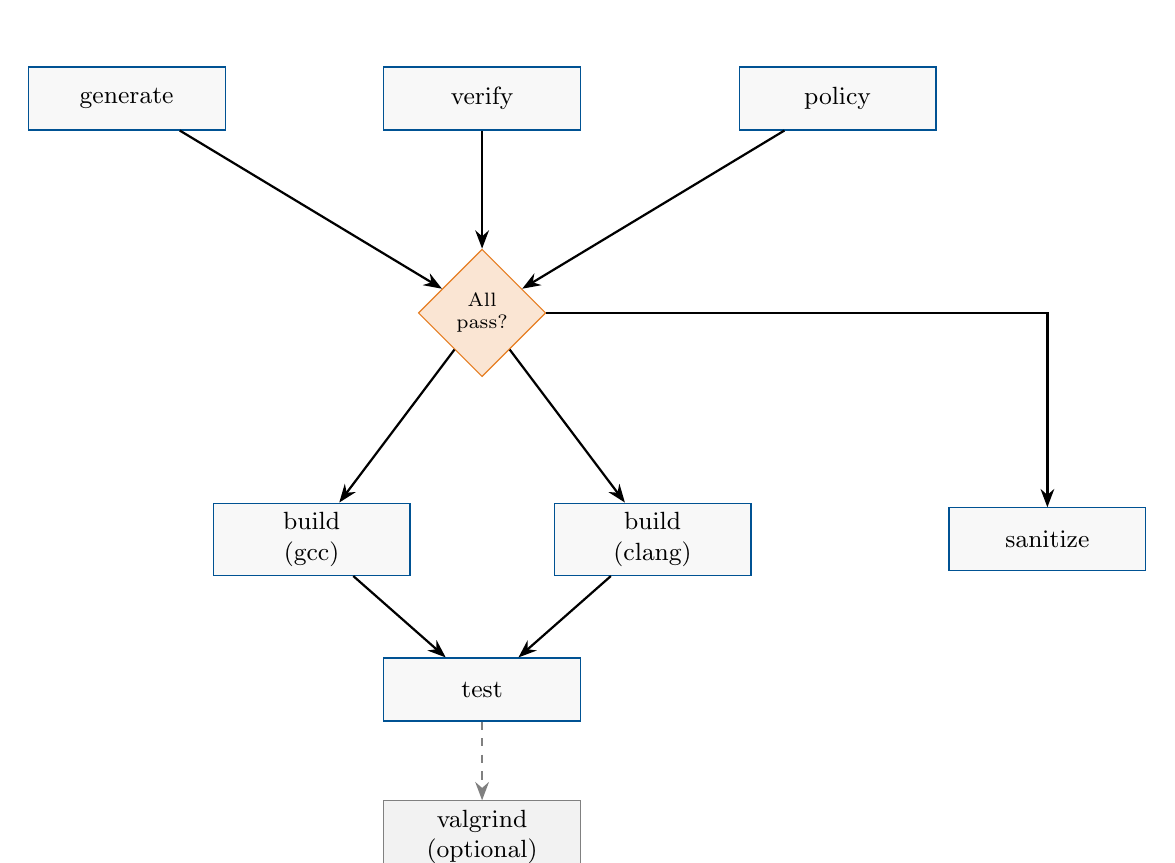
\begin{tikzpicture}[
    node distance=1.2cm and 2cm,
    job/.style={rectangle, draw=primaryblue, fill=lightgray, 
                minimum width=2.5cm, minimum height=0.8cm, 
                font=\small, align=center},
    gate/.style={diamond, draw=accentorange, fill=accentorange!20,
                minimum width=1cm, minimum height=1cm,
                font=\scriptsize, align=center},
    arrow/.style={-{Stealth}, thick}
]
    % First row - parallel gates
    \node[job] (gen) {generate};
    \node[job, right=of gen] (verify) {verify};
    \node[job, right=of verify] (policy) {policy};
    
    % Gate
    \node[gate, below=1.5cm of verify] (gate1) {All\\pass?};
    
    % Second row - parallel builds
    \node[job, below left=2cm and 0.5cm of gate1] (build-gcc) {build\\(gcc)};
    \node[job, below right=2cm and 0.5cm of gate1] (build-clang) {build\\(clang)};
    \node[job, right=2.5cm of build-clang] (sanitize) {sanitize};
    
    % Third row
    \node[job, below=1.5cm of $(build-gcc)!0.5!(build-clang)$] (test) {test};
    
    % Optional
    \node[job, below=1cm of test, draw=gray, fill=gray!10] (valgrind) {valgrind\\(optional)};
    
    % Arrows
    \draw[arrow] (gen) -- (gate1);
    \draw[arrow] (verify) -- (gate1);
    \draw[arrow] (policy) -- (gate1);
    
    \draw[arrow] (gate1) -- (build-gcc);
    \draw[arrow] (gate1) -- (build-clang);
    \draw[arrow] (gate1) -| (sanitize);
    
    \draw[arrow] (build-gcc) -- (test);
    \draw[arrow] (build-clang) -- (test);
    
    \draw[arrow, dashed, gray] (test) -- (valgrind);
\end{tikzpicture}
\caption{CI Job Dependency Graph}
\label{fig:job-deps}
\end{figure}

\chapter{Troubleshooting}
\label{app:troubleshooting}

\section{Common Failures}
\label{sec:common-failures}

\begin{definitionbox}{ooc/verify fails: ``Public headers contain struct bodies''}
\textbf{Cause:} A public header in \filepath{src/ooc/include/} contains a \code{struct \{ ... \}} definition.

\textbf{Fix:} Move the struct definition to a private header in \filepath{src/ooc/internal/}. The public header should only contain:
\begin{lstlisting}[language=C,numbers=none]
typedef struct MyClass MyClass;  // Opaque declaration
\end{lstlisting}
\end{definitionbox}

\begin{definitionbox}{ooc/policy fails: ``Class X missing method specification''}
\textbf{Cause:} A \code{.d} file exists without a corresponding \code{.ms} file.

\textbf{Fix:} Create the missing method specification file:
\begin{lstlisting}[language=bash,numbers=none]
touch src/ooc/classes/MyClass.ms
\end{lstlisting}
\end{definitionbox}

\begin{definitionbox}{ooc/sanitize fails: ``heap-use-after-free''}
\textbf{Cause:} Object accessed after \code{delete} was called.

\textbf{Fix:} Review object lifecycle. Common causes:
\begin{itemize}
    \item Deleting base pointer but continuing to use derived pointer
    \item Missing NULL assignment after delete
    \item Incorrect destructor chain
\end{itemize}
\end{definitionbox}

\begin{definitionbox}{Compile error: ``static assertion failed: vtable must be first''}
\textbf{Cause:} Structure definition has fields before the class pointer.

\textbf{Fix:} Ensure the \code{const struct Class* class} field is first:
\begin{lstlisting}[language=C,numbers=none]
struct MyClass {
    const struct Class* class;  // MUST be first
    // other fields follow
};
\end{lstlisting}
\end{definitionbox}

%% =============================================================================
%% BIBLIOGRAPHY / INDEX (if needed)
%% =============================================================================

\chapter{References}
\label{app:references}

\begin{enumerate}[leftmargin=*]
    \item Schreiner, Axel-Tobias. \textit{Object-Oriented Programming in ANSI C}. Hanser, 1993.
    \item GitHub Actions Documentation: \url{https://docs.github.com/en/actions}
    \item Open Policy Agent: \url{https://www.openpolicyagent.org/docs/latest/}
    \item AddressSanitizer: \url{https://clang.llvm.org/docs/AddressSanitizer.html}
    \item Valgrind Manual: \url{https://valgrind.org/docs/manual/}
\end{enumerate}

\end{document}
